\section{Schulklassenvideo}
\label{Schulvideo}
Zur Visualisierung der Problematik der Daten, wurde ein anderes Bild verwendet, da aus Datenschutzgründen kein originales Bild des Unterrichtes veröffentlicht werden darf. Die Bildaufteilung, Kameraausrichtung und Auflösung des Datensatzes ist ähnlich zur \autoref{fig:schulklasse}. Zur Verfügung steht nur ein einfaches Video der Schulklasse, ohne Ground-Truth Daten. Außerdem wurde es mit einer unbekannten Videokamera aufgezeichnet, daher sind nur die Parameter des Filmes $(640 \times 480$ Pixel mit $25Fps)$ bekannt.
\newpage
Die Hauptproblematik ist die Bildauflösung, sie ist sehr gering und die Gesichter sind nur durch entsprechend wenige Pixel dargestellt. Außerdem ist die Distanz zwischen Schülern und Kamera sehr unterschiedlich wodurch verscheiden Größen entstehen.\\
\begin{figure}
	\centering
	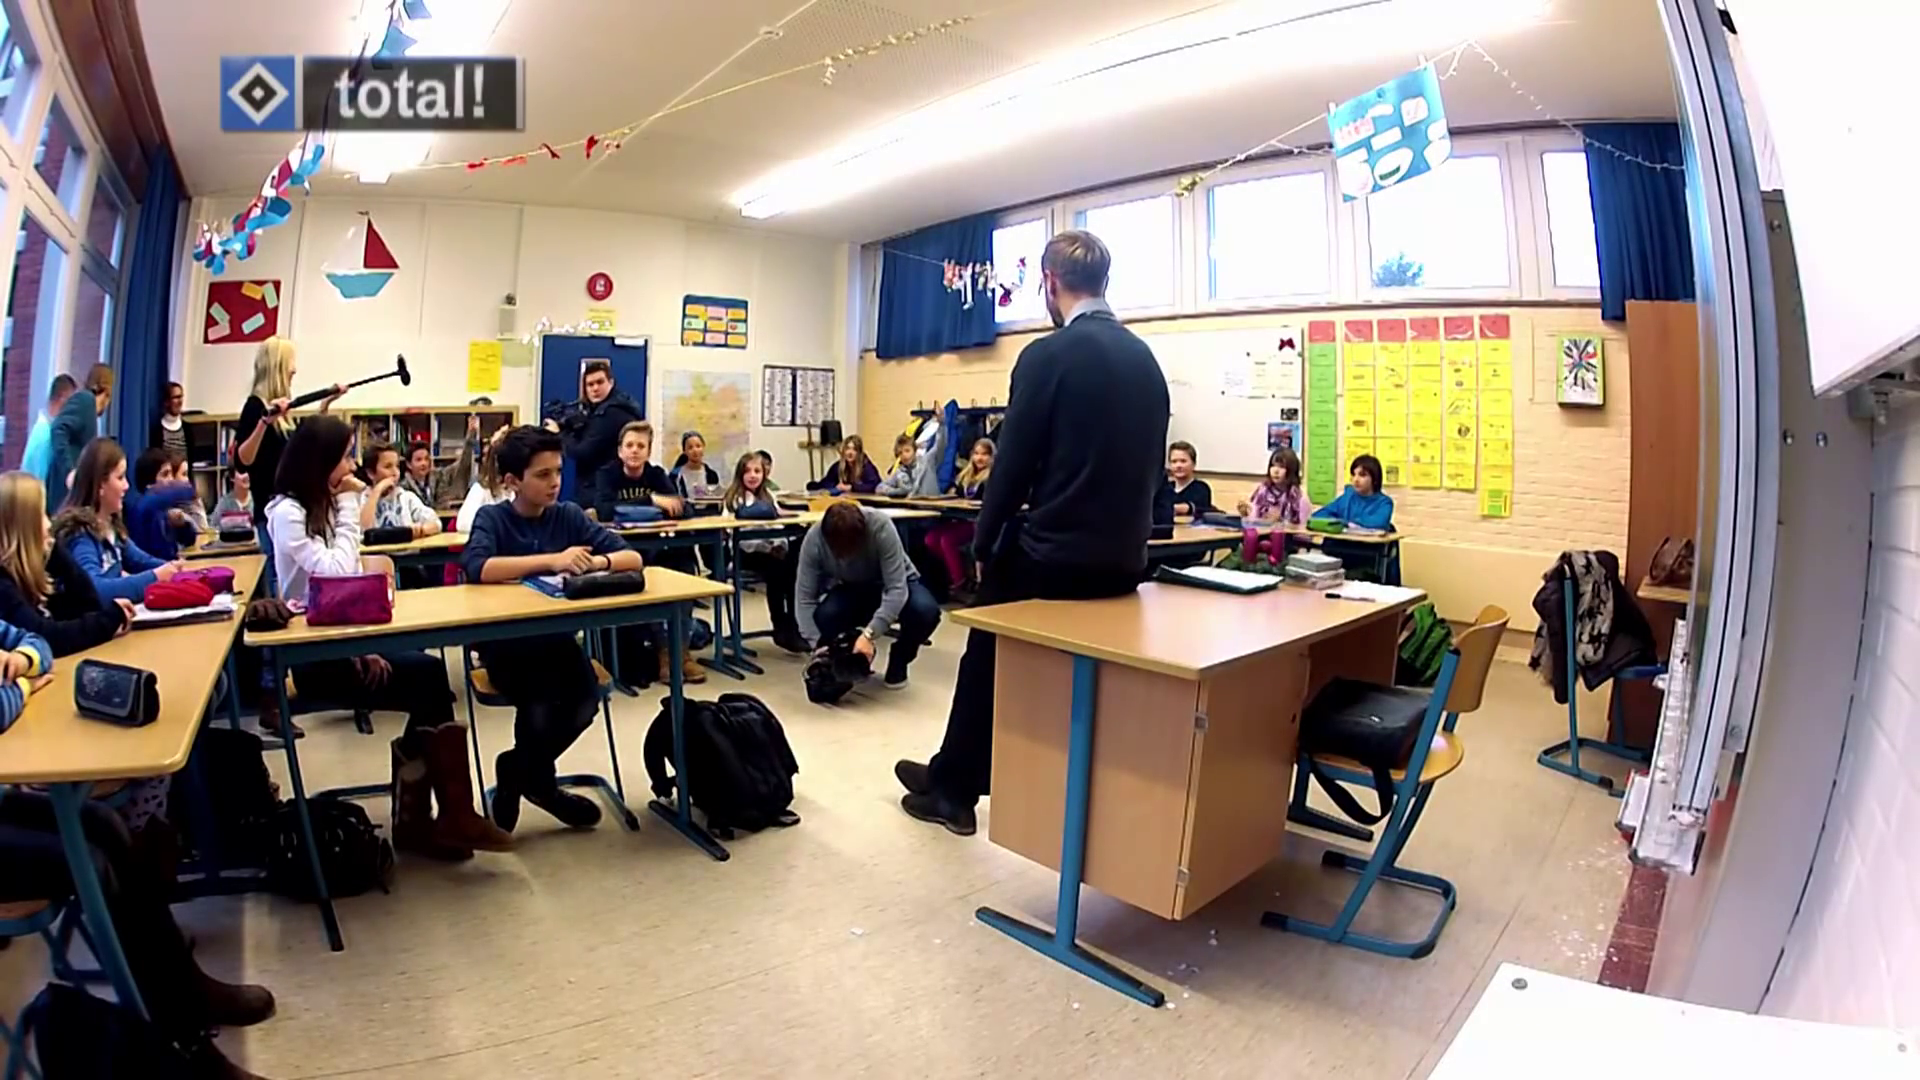
\includegraphics[width=\linewidth]{img/Schulklasse}
	\caption{Beispielhaftes Bild eines Klassenzimmers mit einer ähnlichen Szene wie sie auch im Datensatz vorhanden ist. Bildquelle \cite{Schulklasse_Video}}
	\label{fig:schulklasse}
\end{figure}
